\section* {1.1  LU -  разложение матриц}

\subsection{Постановка задачи}
Реализовать алгоритм LU -  разложения матриц (с выбором главного элемента) в виде программы. Используя разработанное программное обеспечение, решить систему линейных алгебраических уравнений (СЛАУ). Для матрицы СЛАУ вычислить определитель и обратную матрицу. 

{\bfseries Вариант:} 26

\begin{cases}
& -2x_1-9x_2-3x_3+7x_4 = -26 \\
& -7x_1+8x_2+2x_3+5x_4 = -25 \\
& -6x_1+2x_2 = -16 \\
& -3x_2+8x_3-3x_4 = -5 \\
\end{cases}
%\pagebreak

\subsection{Результаты работы}
\begin{figure}[h!]
\centering
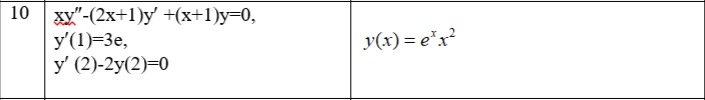
\includegraphics[width=15cm, height=10cm]{img1}
\caption{Вывод программы в консоли}
\end{figure}
\pagebreak

\subsection{Исходный код}
Общие файлы для всех подзадач 1 лабораторной работы:
\lstinputlisting{include/lab1.h}
\lstinputlisting{include/lab1.c}
Коэффициенты перед иксами системы:
\lstinputlisting{include/lab1-1m.txt}
Вектор b:
\lstinputlisting{include/lab1-1v.txt}
\lstinputlisting{include/lab1-1.c}
\pagebreak
\section* {1.2  Метод прогонки}

\subsection{Постановка задачи}
Реализовать метод прогонки в виде программы, задавая в качестве входных данных ненулевые элементы матрицы системы и вектор правых частей. Используя разработанное программное обеспечение, решить СЛАУ с трехдиагональной матрицей.  

{\bfseries Вариант:} 26

\begin{cases}
& -12x_1-7x_2 = -102 \\
& -7x_1-11x_2-3x_3 = -92 \\
& -7x_2+21x_3-8x_4= -65 \\
& 4x_3-13x_4+5x_5 = 38 \\
& -6x_4+14x_5 = -12\\
\end{cases}
% \pagebreak

\subsection{Результаты работы}
\begin{figure}[h!]
\centering
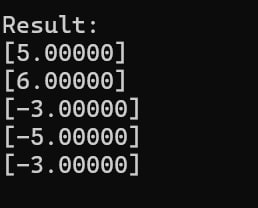
\includegraphics[width=.7\textwidth]{img2}
\caption{Вывод программы в консоли}
\end{figure}
\pagebreak

\subsection{Исходный код}
Коэффициенты перед исками системы:
\lstinputlisting{include/lab1-2m.txt}
Вектор b:
\lstinputlisting{include/lab1-2v.txt}
\lstinputlisting{include/lab1-2.c}
\pagebreak
\section* {1.3  Метод простых итераций. Метод Зейделя}

\subsection{Постановка задачи}
Реализовать метод простых итераций и метод Зейделя в виде программ, задавая в качестве входных данных матрицу системы, вектор правых частей и точность вычислений. Используя разработанное программное обеспечение, решить СЛАУ. Проанализировать количество итераций, необходимое для достижения заданной точности. 

{\bfseries Вариант:} 26

\begin{cases}

& 18x_1-2x_3+7x_4 = 50 \\
& -x_1+14x_2-3x_3+2x_4 = 2 \\
& 5x_1+5x_2+26x_3+7x_4 = 273 \\
& -2x_1-6x_2+9x_3+24x_4 = 111 \\
\end{cases}
% \pagebreak

\subsection{Результаты работы}
\begin{figure}[h!]
\centering
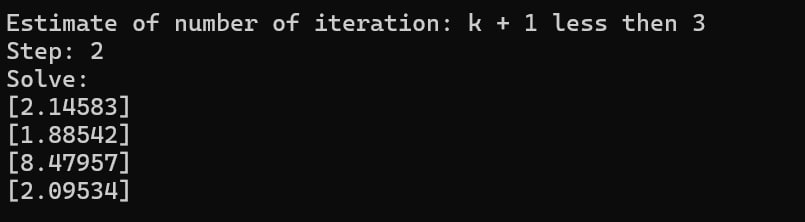
\includegraphics[width=15cm, height=10cm]{img3}
\caption{Вывод программы в консоли}
\end{figure}

% \vfill

\pagebreak

\subsection{Исходный код}
Эпсилон:
\lstinputlisting{include/lab1-3e.txt}
Коэффициенты перед иксами системы:
\lstinputlisting{include/lab1-3m.txt}
Вектор b:
\lstinputlisting{include/lab1-3v.txt}
\lstinputlisting{include/lab1-3.c}
\pagebreak
\section* {1.4  Метод вращений}

\subsection{Постановка задачи}
Реализовать метод вращений в виде программы, задавая в качестве входных данных матрицу и точность вычислений. Используя разработанное программное обеспечение, найти собственные значения и собственные векторы симметрических матриц. Проанализировать зависимость погрешности вычислений от числа итераций. 

{\bfseries Вариант:} 26

  \begin{pmatrix}
    -4 & 1 & -7 \\
    1 & 9 & 1 \\
    -7 & 1 & 7
  \end{pmatrix}
% \pagebreak

\subsection{Результаты работы}
\begin{figure}[h!]
\centering
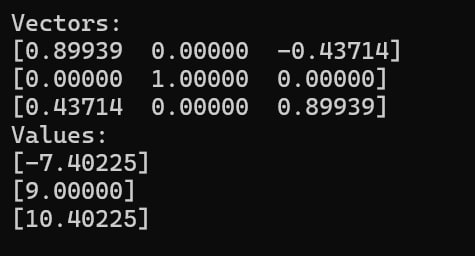
\includegraphics[width=.9\textwidth]{img4}
\caption{Вывод программы в консоли}
\end{figure}

\pagebreak

\subsection{Исходный код}
Эпсилон:
\lstinputlisting{include/lab1-4e.txt}
Матрица:
\lstinputlisting{include/lab1-4m.txt}
\lstinputlisting{include/lab1-4.c}
\pagebreak
\section* {1.5  QR – разложение матриц}

\subsection{Постановка задачи}
Реализовать алгоритм QR – разложения матриц в виде программы. На его основе разработать программу, реализующую QR – алгоритм решения полной проблемы собственных значений произвольных матриц, задавая в качестве входных данных матрицу и точность вычислений. С использованием разработанного программного обеспечения найти собственные значения матрицы.


{\bfseries Вариант:} 26

  \begin{pmatrix}
    -9 & -9 & -3 \\
    -9 & 0 & -2 \\
    -5 & -1 & -4
  \end{pmatrix}
% \pagebreak

\subsection{Результаты работы}
\begin{figure}[h!]
\centering
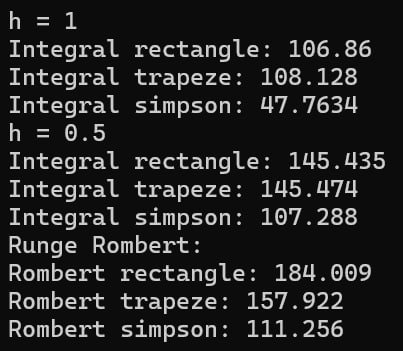
\includegraphics[width=.9\textwidth]{img5}
\caption{Вывод программы в консоли}
\end{figure}

\pagebreak

\subsection{Исходный код}
Эпсилон:
\lstinputlisting{include/lab1-5e.txt}
Матрица:
\lstinputlisting{include/lab1-5m.txt}
\lstinputlisting{include/lab1-5.c}